\subsection{Abstract reduction systems}

\begin{definition}[Abstract reduction system]
Given a set $A$ and a binary relation $\to$ in $A$.

An abstract reduction system is a pair $(A,\to)$. The binary relation $\to$ can be seen to represent computation steps. 

We note $(a,b) \in \to$ as $a \to b$. 
\end{definition}

We want to determine if two terms are equivalent, that is, if $a \stackrel{*}{\leftrightarrow} b$. Our strategy is the one that we pointed out in the examples about groups: to reduce to a certain normal form that has a uniqueness property. The advantage of this approach is that an undirected search on $\to$ and $\gets$ would be too expensive. First we need some notation for operations that are based on the composition of relations: 

Given $R \subseteq A \times B \land S \subseteq B \times C$ two relations, its composition is: $$R \circ S = \{(x,z) \in A \times C: \exists y \in B. (x,y) \in R \land (y,z) \in S\}$$

\begin{table}[H]
\centering
\begin{adjustwidth}{-2cm}{}
\begin{tabular}{|| c | c | c | c ||}
\hline
\hline & $\stackrel{0}{\rightarrow} = \{(x,x):x \in A \}$ & & $\stackrel{i+1}{\rightarrow} = \stackrel{i}{\rightarrow} \circ \to$ \\
\hline Transitive closure & $\stackrel{+}{\rightarrow} = \cup_{i > 0} \stackrel{i}{\rightarrow}$ & Reflexive transitive closure & $\stackrel{*}{\rightarrow} = \stackrel{+}{\rightarrow} \cup \stackrel{0}{\rightarrow}$ \\
\hline  Reflexive closure & $\stackrel{=}{\rightarrow} = \to \cup \stackrel{0}{\rightarrow}$ & Inverse & $\stackrel{-1}{\rightarrow} = \{(y,x):x \to y\}$ and $\leftarrow= \stackrel{-1}{\rightarrow}$ \\
\hline  Symmetric closure & $\leftrightarrow = \to \cup \leftarrow$ & Transitive symmetric closure & $\stackrel{+}{\rightarrow} = (\leftrightarrow)^+$ \\
\hline Reflexive, transitive, symmetric closure &  $\stackrel{*}{\rightarrow} = (\leftrightarrow)^*$ & & \\
\hline
\end{tabular}
\end{adjustwidth}
\caption{Notation for operations on relations}
\label{table:notation1}
\end{table}

We give some terminology for abstract reduction systems:

\begin{table}[H]
\centering
\begin{tabular}{|| c | c | c | c ||}
\hline
\hline x is reducible & $\exists y. x \to y$ & 
x is irreducible or in normal form  & $!\exists y. x \to y$ \\
\hline y is a normal form of x & $x \stackrel{*}{\rightarrow} y \land y$ is in normal form & unique normal form of x (if exists) & $x\downarrow$ \\
\hline y is direct successor of x & $x \to y$ &
y is successor of x & $x \stackrel{+}{\rightarrow} y$ \\
\hline x and y are joinable & $\exists z \in x \stackrel{*}{\rightarrow} z \stackrel{*}{\leftarrow} y$ & x,y joinable & $x \downarrow y$ \\
\hline
\end{tabular}
\caption{Terminology for the elements of the reduction system}
\label{table:notation2}
\end{table}


And some terminology for reductions:

\begin{table}[H]
\centering
\begin{adjustwidth}{-2cm}{}
\begin{tabular}{|| c | c | c | c ||}
\hline
\hline Church-Rosser & $x \stackrel{*}{\leftrightarrow} y \implies x \downarrow y$ & Semi-confluent & $y_1 \leftarrow x \stackrel{*}{\rightarrow} y_2 \implies y_1 \downarrow y_2$ \\
\hline Confluent & $y_1 \stackrel{*}{\leftarrow} x \stackrel{*}{\rightarrow} y_2 \implies y_1 \downarrow y_2$ & Terminating & there is no infinite descending chain $a_0 \to a_1 \to \cdots$ \\
\hline Normalizing & every element has a normal form & Convergent & confluent and terminating \\
\hline
\end{tabular}
\end{adjustwidth}
\caption{Terminology for reductions in reductions systems}
\label{table:notation3}
\end{table}

\begin{figure}[H]
\centering
\begin{tikzcd}
x \arrow[rr, leftrightarrow, "*"] \arrow[dr, dashrightarrow, "*"'] 
 &  & y \arrow[dl, dashrightarrow, "*"] \\
 & z &
\end{tikzcd}
\begin{tikzcd}
x \arrow[r, "*"] \arrow[d, "*"'] 
&  y_1 \arrow[d, dashed, "*"] \\
y_2 \arrow[r, dashed, "*"] & z
\end{tikzcd}
\begin{tikzcd}
x \arrow[r] \arrow[d, "*"] 
&  y_1 \arrow[d, dashed, "*"] \\
y_2 \arrow[r, dashed, "*"] & z
\end{tikzcd}
\caption{Church-Rosser, confluence and semi-confluence diagrams}
\end{figure}

\begin{proposition}[Relation between the properties of an abstract reduction system] 
The following propositions relate the properties of abstract reduction systems:

\begin{enumerate}
\item Any terminating relation is normalizing. The converse is not true. 
\item Church-Rosser $\iff$ Confluence $\iff$ Semi-confluence. 
\item Given a confluent relation $\to$ and $x \stackrel{*}{\leftrightarrow} y$:

1. y is in normal form $ \implies x \stackrel{*}{\rightarrow} y$\\
2. x,y are in normal form $ \implies x = y$. 
\end{enumerate}
\end{proposition}
\begin{proof}
\begin{enumerate}
\item Clearly, every terminating relation arrives to a normal form from any initial term. For the converse, consider the following acyclic, confluent and non-terminating relation:

\begin{tikzcd}
\cdot \arrow[r] \arrow[d] 
&  \cdot \arrow[r] \arrow{dl} 
& \cdot \arrow{dll} \arrow{r}
& \cdot \arrow{dlll}
& \cdots \\
\cdot 
\end{tikzcd}

\item 1) $\implies$ 2). Assume $y_1 \stackrel{*}{\leftarrow} x \stackrel{*}{\rightarrow} y_2$ then $x \stackrel{*}{\leftrightarrow} y$ and by Church-Rosser $\exists y_1 \downarrow y_2$.

2) $\implies$ 3). Trivial.

3) $\implies$ 1). Assume $x \stackrel{*}{\leftrightarrow} y$. By induction, if $x = y$ then $x \downarrow y$. Assuming $x \stackrel{*}{\leftrightarrow} y \leftrightarrow y'$ and that $x \downarrow y$ we need to show $x \downarrow y'$. There are two cases:

\begin{tikzcd}
& & & y' \arrow{dl} \\
 x  \arrow[rr, leftrightarrow, "*"] \arrow[dr,dashed,"*"] & & y \arrow[dl,dashed,"*"] \\
& \cdot
\end{tikzcd} \hspace{3mm}
\begin{tikzcd}
x \arrow[rr,leftrightarrow,"*"] \arrow[dr,dashed,"*",swap] & & y \arrow[dr] \arrow[dl,dashed,"*"] \\
& z \arrow[dr,dashed,"*",swap] & & y' \arrow[dl,dashed,"*",swap] \\
& & \cdot
\end{tikzcd}

For the first case, we perform induction on the lower triangle and in the second, induction on the upper triangle and then semi-confluence for the quadrilateral.

\item We take advantage of the fact that confluence is equivalent to Church Rosser and consider the following diagrams:

\begin{tikzcd}
x \arrow[rr,leftrightarrow,"*"] \arrow[rr,bend right]  & & y 
\end{tikzcd} \hspace{3mm}
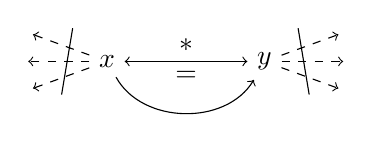
\begin{tikzpicture}

\node (x) at (0,0) {$x$};
\node (y) at (2,0) {$y$};

\draw[<->] (x) -- node[above] {$\ast$} node[below] {$=$} (y);
\draw[->] (x) to[bend right=60] (y);

\draw[->,dashed] (x) -- +(160:1);
\draw[->,dashed] (x) -- +(180:1);
\draw[->,dashed] (x) -- +(200:1);

\draw[->,dashed] (y) -- +(20:1);
\draw[->,dashed] (y) -- +(0:1);
\draw[->,dashed] (y) -- +(-20:1);

\draw ([yshift=12,xshift=-6]x.west) -- ([yshift=-12,xshift=-10]x.west);
\draw ([yshift=12,xshift=6]y.east) -- ([yshift=-12,xshift=10]y.east);

\end{tikzpicture}
\end{enumerate}
\end{proof}

\begin{proposition}[Results on the reduction strategy]
The following results give us hints on what conditions should we look for to apply the strategy of our motivation:

\begin{enumerate}
\item Condition for well-definition of $x\downarrow$:

\begin{enumerate}
\item $\to$ is confluent $\implies$ every element has at most one normal form.
\item $\to$ is normalizing and confluent $\implies$ every element has a unique normal form.
\end{enumerate}

\item Equivalence test with normal forms:

If $\to$ is confluent and normalizing then $x \stackrel{*}{\leftrightarrow} y \iff x\downarrow = y\downarrow$

\item Equivalence test with normal forms:

If $\to$ is convergent then $x \stackrel{*}{\leftrightarrow} y \iff x\downarrow = y\downarrow$
\end{enumerate}
\end{proposition}
\begin{proof}
\begin{enumerate}
\item 

\begin{enumerate}
\item If x has two normal forms $n_1^x,n_2^x$ by confluence we can join them. But since they're normal the only way to join them is that they are equal.
\item Use 1 to proof that the number of normal forms is $\le 1$ and normality to proof that it is $\ge 1$.
\end{enumerate}

\item $x \stackrel{*}{\leftrightarrow} y \implies x \downarrow \stackrel{*}{\leftrightarrow} y \implies x \downarrow \implies x \downarrow = y \downarrow$.

$x \downarrow = y \downarrow \implies x \stackrel{*}{\leftrightarrow} y$

\begin{tikzcd}
x \arrow[r,leftrightarrow,"*"] \arrow[d,leftrightarrow,"*",swap] & 
y \arrow[d,leftrightarrow,"*",swap] \\
x \downarrow \arrow[r,leftrightarrow,dashed,"*"] & y \downarrow
\end{tikzcd}

\item This a weaker result than the previous but note that in the search for normal forms, the previous one requires a breadth-first search which may be more costly in some situations. Therefore, literature focus on the convergent case. 
\end{enumerate}
\end{proof}


So now the question is, how do we prove confluence and termination?

\subsubsection{Termination}

Well-founded induction is a first tool to prove termination. It is a generalization of strong induction for natural numbers:

\begin{definition}[Strong induction for natural numbers]
Given property $P$ on natural numbers. 

$\forall n \in \mathbb{N}. P(n) \iff \forall n \in \mathbb{N}. (\forall m \in \mathbb{N}. m < n \implies P(m)) \implies P(n)$.
\end{definition}

Note that the base case for $0$ leaves the right hand-side with proving $P(0)$ just what we do in normal induction proofs. Now we abstract this principle from $(\mathbb{N},>)$ to any reduction system $(A,\to)$:

\begin{definition}[Well-founded induction (WFI) rule]
Given a property $P$ on the elements of $A$:\\

\infer{\forall x \in A. P(x)}{\forall x \in A. (\forall y \in A. x \stackrel{+}{\rightarrow} y \implies P(y)) \implies P(x)}
\end{definition}

In this case, the base case reduces to prove $P(x)$ for every $x$ without successor. It is interesting that this property holds exactly for terminating relations.

\begin{theorem}[Characterization of terminating relations]
Given $(A,\to)$ an abstract reduction system. 

WFI holds $\iff$ $\to$ terminates $\iff \forall B \subseteq A.\exists b \in B. \nexists b' \in B.b \to b'$
\end{theorem}
\begin{proof}
$\Rightarrow)$ Set $P(x) = $ there is no infinite chain starting from x. Given any $x$ the premise of WFI says that no successor of x has an infinite chain. Therefore, $x$ itself cannot have an infinite chain. Equivalently, $P(x)$ holds. 

$\Leftarrow)$ If WFI doesn't hold for $\to$ then there must exist $a_0 \in A$ such that: $$[\forall y \in A. a_0  \stackrel{+}{\rightarrow} y \implies P(y)) \implies P(a_0)] \land \lnot P(a_0)$$ Therefore there must exist $a_1 \in A$ such that: $$a_0 \stackrel{+}{\rightarrow} a_1 \land \lnot P(a_1)$$ This process repeats itself giving a chain: $$a_0 \stackrel{+}{\rightarrow} a_1 \stackrel{+}{\rightarrow} \cdots$$ that does not terminate.
\end{proof}

\begin{definition}[Properties related to termination]
A relation $\to$ is called:

\begin{enumerate}
\item \textbf{finitely branching} if each element has only a finite number of direct successors.
\item \textbf{globally finite} if each element has only finitely many successors.
\item \textbf{acyclic} if there is no element a such that $a \stackrel{+}{\rightarrow} a$. 
\end{enumerate}
\end{definition} 

\begin{proposition}[Relation between properties related to termination]
1. $\to$ terminating and finitely branching $\implies$ globally finite. \\
2. $\to$ acyclic and globally finite $\implies$ terminating. \\
3. $\to$ acyclic and finitely branching $\implies$ (globally finite $\iff$ terminating) \\
4. K\"onig's lemma: a finitely branching tree is infinite $\iff$ it contains an infinite path.
\end{proposition}

Different techniques to prove termination are presented in \cite{term-rewriting}. They imply the use of many orders such as lexicographic or multi-set orders which do not convey our main goal here of presenting general concepts towards completion algorithms. There is also an interesting comment on the characterization of termination with monotonic embeddings in $(\mathbb{N},>)$ for finitely branching relations.

\subsubsection{Confluence}

We now look at techniques to prove confluence. 

\begin{definition}[Other notions of confluence]
$\to$ is locally confluent $\iff \forall y_1,y_2 \in A. y_1 \gets x \to y_2 \implies y_1 \downarrow y_2$

$\to$ is strongly confluent $\iff \forall y_1,y_2,x.y_1 \gets x \to y_2 \implies \exists z.y_1 \stackrel{*}{\to} z \stackrel{=}{\gets} y_2$

$\to$ has the diamond property $\iff \forall y_1,y_2,x. y_1 \gets x \to y_2 \implies \exists z. y_1 \to z \gets y_2$
\end{definition}

Note that local confluence does not imply confluence as in the following example:

\begin{tikzcd} 
a  & 0 \arrow[r,bend left] \arrow[l] & 1 \arrow[r] \arrow[l,bend left] & b 
\end{tikzcd}

Note also that the diamond property is stronger than strong confluence. 

It is clear also that $\to$ is confluent $\iff$ $\stackrel{*}{\to}$ has the diamond property.

\begin{proposition}[Sufficient conditions for confluence]
The following are sufficient conditions to show confluence:

\begin{enumerate}
\item Newman's lemma: $\to$ terminating and locally confluent $\implies$ confluent.

\item $\to$ strongly confluent $\implies$ confluent.

\end{enumerate}
\end{proposition}
\begin{proof}
\begin{enumerate}
\item Well-founded induction on $P(x) = \forall y,z.y \stackrel{*}{\gets} x \stackrel{*}{\to} z \implies y \downarrow z$. We analyse $y \stackrel{*}{\gets} x \stackrel{*}{\to} z$:

\begin{enumerate}
\item If $x = y \lor x = z$ then $y \downarrow z$. 
\item In other case, $x \to y_1 \stackrel{*}{y} \land x \to z_1 \stackrel{*}{\to} z \stackrel{\text{local confluence}}{\implies} \exists u = y_1 \downarrow z_1$.

Since $x \stackrel{+}{\to} y_1 \land x \stackrel{+}{z_1} \stackrel{\text{ induction }}{\implies} \exists v = y \downarrow u \land w = v \downarrow z \implies \exists w = y_1 \downarrow z_1$
\end{enumerate}

\begin{tikzcd}
& & x \arrow[dl] \arrow[dr] & & \\
& y_1 \arrow[dl,"*",swap] \arrow[dr,dashed,"*"] & & z_1 \arrow[dl,dashed,"*",swap] \arrow[dr,"*"] & \\
y \arrow[dr,dashed,"*"] & & u \arrow[dl,dashed,"*",swap] & & z \arrow[ddll,dashed,"*",swap] \\
& v \arrow[dr,dashed,"*"] & & & \\
& & w & &
\end{tikzcd}

\item We prove semi-confluence with $y_1 \gets x_1 \stackrel{n}{\to} x_n \implies \exists y_n.y_1 \stackrel{*}{\to} y_n \stackrel{=}{\gets} x_n$ and we apply induction over $n$.

\begin{tikzcd} 
x_1 \arrow[r] \arrow[d] & x_2 \arrow[d,dashed,"="] & \ldots & x_{n-1} \arrow[d,dashed,"="] \arrow[r] & x_n \arrow[d,dashed,"="] \\
y_1 \arrow[r,dashed,"*"] & y_2  & \ldots & y_{n-1} \arrow[r,dashed,"="] & y_n
\end{tikzcd}
\end{enumerate}
\end{proof}

To use strong confluence property one defines given a relation $\to$, a stronly confluent relation $\to_s$ such that $\stackrel{*}{\to} = \stackrel{*}{\to_s}$ and by the theorem above we have that $\to$ is confluent ($\stackrel{*}{\to} = \stackrel{*}{\to_s} \implies \to_1 \text{ confluent } \iff \to_2 \text{ confluent }$). A sufficient condition for $\stackrel{*}{\to_1} = \stackrel{*}{\to_2}$ is $\to_1 \subseteq \to_2 \subseteq \stackrel{*}{\to_1}$. Therefore we have the following:

\begin{corollary}[Proving confluence by strong confluence]
If $\to_1 \subseteq \to_2 \subseteq \stackrel{*}{\to_1}$ and $\to_2$ is strongly confluent then $\to_1$ is confluent. 
\end{corollary}

Another strategy may be to split $\to = \to_1 \cup \to_2$ and prove that the confluence of each part gives the confluence of the total. The following concept is useful to prove this implication:

\begin{definition}[Commutation]
Two relations $\to_1,\to_2$:

\begin{enumerate}
\item commute: $\forall y_1,y_2,x.y_1 \stackrel{*}{\gets_1} x \stackrel{*}{\to_2} y_2 \implies \exists z.y_1 \stackrel{*}{\to_2} z \stackrel{*}{\gets_1} y_2 \iff \stackrel{*}{\gets_1} \circ \stackrel{*}{\to_2} \subseteq \stackrel{*}{\to_2} \circ \stackrel{*}{\gets_1}$
\item strongly conmute: $\forall y_1,y_2,x.y_1 \gets_1 x \to_2 y_2 \implies \exists z.y_1 \stackrel{=}{\to_2} z \stackrel{*}{\gets_1} y_2 \iff \gets_1 \circ \to_2 \subseteq \stackrel{=}{\to_2} \circ \stackrel{*}{\gets_1}$
\end{enumerate}
\end{definition}

\begin{proposition}[Commutation properties]
1. Commutation Lemma: If $\to_1,\to_2$ commute strongly then they commute.\\
2. Commutative Union Lemma: If $\to_1,\to_2$ are confluent and commute then $\to_1 \cup \to_2$ is confluent. 
\end{proposition}










